\setlength\abovedisplayskip{0.4pt}
\setlength\belowdisplayskip{0.4pt}

\chapter{Ultra-peripheral collisions at the Large Hadron Collider}

In this chapter, I will review recent LHC results on ultra-peripheral collisions (UPCs). First I will discuss the unique features of UPCs, and how they are selected. I then present the results from ALICE and CMS on vector meson photoproduction as an example of how UPCs can probe the nuclear gluon distribution. The ATLAS results for light-by-light scattering are described. The final section explains dijet photoproduction in UPCs, and how the factorisation theorem informs the interpretation of coherent dijet correlations. 

\section{Ultra-peripheral heavy-ion collisions}

Similar to the Rutherford experiment, in heavy-ion collisions the scattered particles carry information about the internal structure of the nucleus. The Rutherford experiment has the three components that still characterize high-energy nuclear experiments: a probe, a medium, and a signal. Alpha particles probe the medium of the gold atom, and the angular distribution of scattered alpha particles signals the internal structure of the atom. 

Ultra-peripheral collisions occur at impact parameters greater than the sum of the heavy-ion radii. In these collisions, hadronic interactions are strongly suppressed while photonuclear activity is enhanced proportional to the square of the nuclear charge \cite{Hands:2001ve}. The electromagnetic field of an incoming heavy-ion, from the perspective of a target, is equivalent to a flux of virtual photons; figure \ref{fig:smushedField} illustrates the Lorentz contraction of the field of a boosted charge \cite{Baltz:2007kq}\cite{WWJackson}.
\begin{figure}[h!]
\begin{centering}
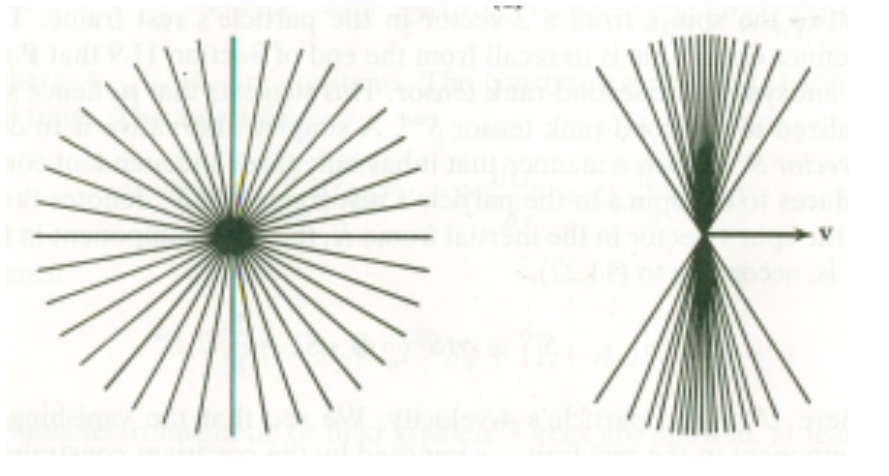
\includegraphics[width=4in]{Chapter1/importfigs/jackson_em_wwa.png}
\par\end{centering}
\caption{ (a.) electromagnetic field of stationary charge (b.) eletromagnetic field of boosted charge \cite{WWJackson} \label{fig:smushedField}}
\end{figure}

UPC models typically address two elements: the photon flux, $N_{\gamma / Pb}$, and the photoproduction cross-section, $\sigma_{\gamma Pb}$. These quantities are related to the UPC cross-section, $\sigma_{PbPb}$, in the following equation,
\begin{equation}
\frac{d \sigma_{PbPb}}{dy} = N_{\gamma/Pb}(y,M)\sigma_{\gamma Pb}(y)+N_{\gamma/Pb}(-y,M)\sigma_{\gamma Pb}(-y),
\end{equation}
where there are two terms to reflect that either heavy-ion can be a source of photons \cite{Bertulani:2005ru}. 

The Weizsacker-Williams appoximation (WWA) calculates the density of photons, about the nucleus, as a function of energy. WWA is a semi-classical formulation. Maxwell's equations are solved for a stationary point charge boosted to an ultra-relativistic velocity. In the target's frame, the Fourier transform of the source field is taken. The Fourier frequency modes are interpreted through the quantum mechanical equation of photon energy. The photon flux as function of energy is given by
\begin{equation}
N(\omega,b) = \frac{\alpha}{\hbar \omega}\left( \frac{Z}{b\beta\pi} \right)^2\left ( \frac{\omega b}{\gamma \nu} \right )K_1^2\left ( \frac{\omega b}{\gamma \nu} \right ) ,
\end{equation}
where $\alpha$ is the QED coupling constant, $\omega$ is the photon energy, $Z$ is the atomic number of the nuclei, $b$ is the impact parameter, $\beta$ is ratio of the nuclei speed to the speed of light, $\gamma$ is the Lorentz boost of the nuclei, $K_1^2$ is a Bessel function, $\nu$ is the photon frequency \cite{WWJackson}.

There are ways to represent the photon flux as solely a function of photon wavelength:
\begin{equation}
n(k) = \frac{2 \alpha Z^2}{\pi}\left [ \xi K_0(\xi) - \frac{\xi^2}{Z}(K_1^2(\xi)-K_0^2(\xi)) \right ]
\end{equation}

Gluons are the particle exchanged in strong interactions. However, gluons themselves carry color charge. By analogy, photons transmit the electromagnetic force, but do not themselves have an electric charge. The gluons are spin-1, meaning that more than one can occupy the same quantum state.

When a quark is scattered from a nucleus, the strong force field lines for a tube between the quark and its counterpart. Given that the strong coupling constant increases with distance the strong interaction gathers potential energy until the threshold for quark production is passed, at which point an anti-quark is generated to screen the ejected quark. These quarks continue to separate from each other and continue the quark generation process. The resulting final state hadron distribution takes the form of a cone centered on the path of the initial quark. 

QCD factorisation describes the diffractive-photoproduction dijet cross-section as the convolution of the partonic cross-section with the diffractive parton distributions. However, factorisation only describes H1 data if the resolved-photon contribution is suppressed. 

The photoproduction cross-section is proportional to the gluon distribution. At low momentum transfer, photons interact electromagnetically, i.e. directly, with partons. High energy, "resolved" photons possess a hadronic structure; instead of directly interacting with the nuclei, these photons fluctuate into mediating quark-antiquark pairs. 

\section{Vector meson photoproduction}

The virtual photons present in UPC can fluctuate into a quark-antiquark pair which can take the form of a low mass meson \cite{lta2011.09}. This meson then interacts with the target nuclei via colorless gluon exchange, emitting a vector meson. If the virtual photon interacts coherently with the target nucleus, this is reflected in the transverse momentum of the vector meson. The vector meson decays into a dilepton pair detectable by CMS \cite{Lappi:2013am}. 

For a given final state $X$, the collision cross section is given as
\begin{equation}
\sigma_X = \int d \omega \frac{n(\omega)}{\omega} \sigma_X^\gamma(\omega),
\end{equation}
where $n(\omega)$ is the number of photons emitted at an energy $\omega$, and $\sigma_X^\gamma(\omega)$ is the photonuclear cross-section of the photon-nucleon interaction. The Weizacker-Williams approximation provides $n(\omega)$. The integral reflects how a state $X$ can result from the interaction of a quasi-real photon of varying energy. 

Ultra-peripheral coherent $J/\Psi$ photoproduction was studied in the ALICE 2011 Pb-Pb data \cite{Abelev:2012ba}. Notice that the cross-section of coherent $J/\Psi$ photoproduction, for $\gamma+p\rightarrow J/\Psi+p$, has a power-law dependence on the photon-proton center-of-mass energy, as seen in figure \ref{fig:aliceData1} \cite{Klein:2017nqo}. This data can be used to measure the gluon distribution as a function of Bjorken-x \cite{pQCD2011.08}. 
\begin{figure}[h!]
\begin{centering}
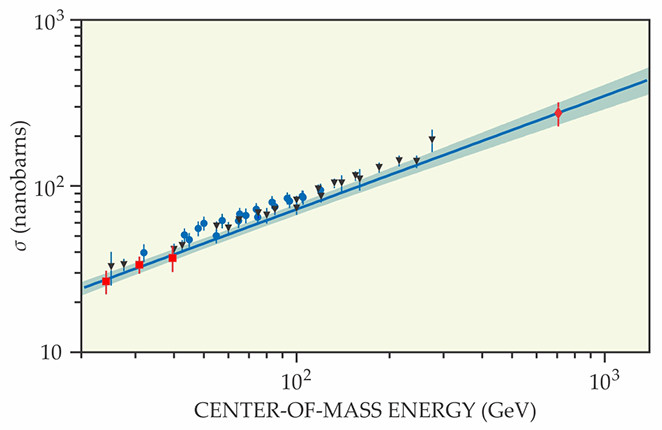
\includegraphics[width=4in]{Chapter2/importfigs/aliceData1.jpeg}
\par\end{centering}
\caption{$\gamma +$proton$\rightarrow J/\Psi +$proton cross-section \cite{Klein:2017nqo}. \label{fig:aliceData1}}
\end{figure}

CMS and ALICE have studied $J/\Psi$ and $\rho$ photoproduction off the proton in proton-Pb collisions \cite{TheALICE:2014dwa}. In coherent UPC photoproduction of $J/\Psi$, the transverse momentum distribution peaks at about 60 MeV because, for coherent production, the photon energy is inversely proportional to the Pb ion diameter, $1/2R_{Pb}$. For this process the photon is interacting with the whole nucleus. The low momentum corresponds to large wavelength of the photon with respect to the nuclear radius \cite{Guzey:2013taa}\cite{Frankfurt:2006wg}. 
\begin{figure}[h!]
\begin{centering}
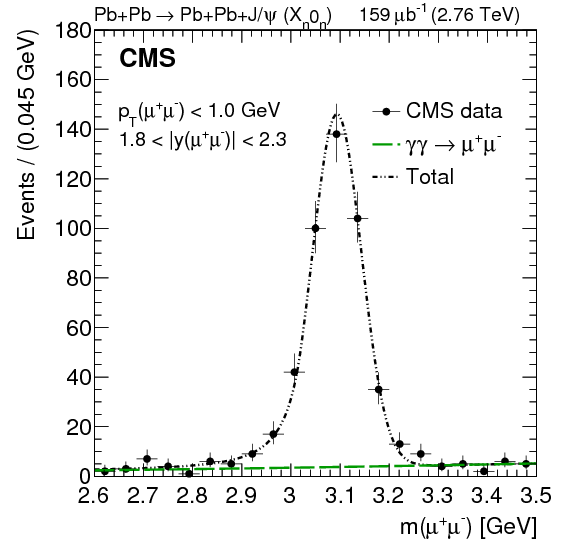
\includegraphics[width=4in]{Chapter2/importfigs/patkenny_Figure_001-a.png}
\par\end{centering}
\caption{Dimuon invariant mass distributions of opposite-sign muon pairs ($p_T<1.0$ GeV, $1.8<|y|<2.3$) \cite{Khachatryan:2016qhq}\label{fig:pk3}}
\end{figure}

UPC vector mesons are a clean probe of the nuclear initial state \cite{Aktas:2006qs}. The high temperature environment of heavy-ion collisions produces a near viscosity free medium that exhibits collective flow. However, collective flow phenomena are also observed in heavy-ion collisions below the QGP phase transition. A good understanding of the heavy-ion initial state, before the phase transition, is necessary to detect authentic QGP pheneomena. UPC productions can probe the initial state because the interaction is purely electromagnetic; hadronic activity is strongly suppressed, excluding the possibility of QGP forming \cite{vmd1999}\cite{vmd2000.03}. 
\begin{figure}[h!]
\begin{centering}
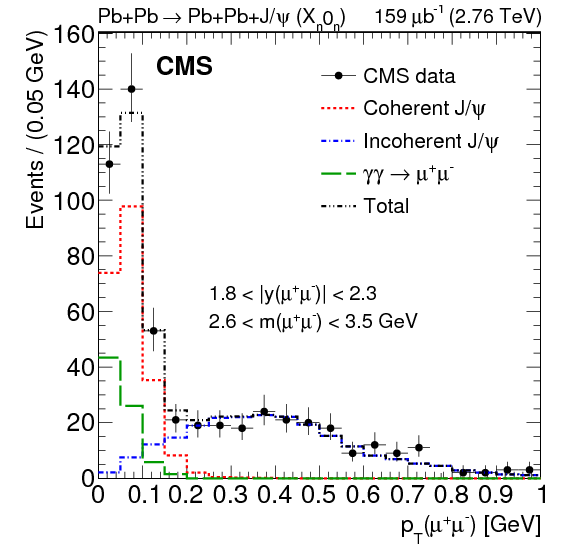
\includegraphics[width=4in]{Chapter2/importfigs/patkenny_Figure_001-b.png}
\par\end{centering}
\caption{Dimuon transverse momentum distributions of opposite-sign muon pairs ($p_T<1.0$ GeV, $1.8<|y|<2.3$) \cite{Khachatryan:2016qhq} \label{fig:pk2}}
\end{figure}

The UPC $J/\Psi$ in particular is senstive to the gluon distribution at low Bjorken-x. The UPC $J/\Psi$ photoproduction cross-section can be calculated from a Glauber model of the heavy-ion \cite{Brodsky:1994kf}. The Glauber model approach depicts the nucleus as a sum of protons and neutrons by scaling up the photon-nuclear cross section derived from electron-proton collisions. Forward neutron tagging was used to separate the coherently and incoherently produced $J/\Psi$ \cite{Guzey:2013jaa} \cite{Strikman:2005ze}.
\begin{figure}[h!]
\begin{centering}
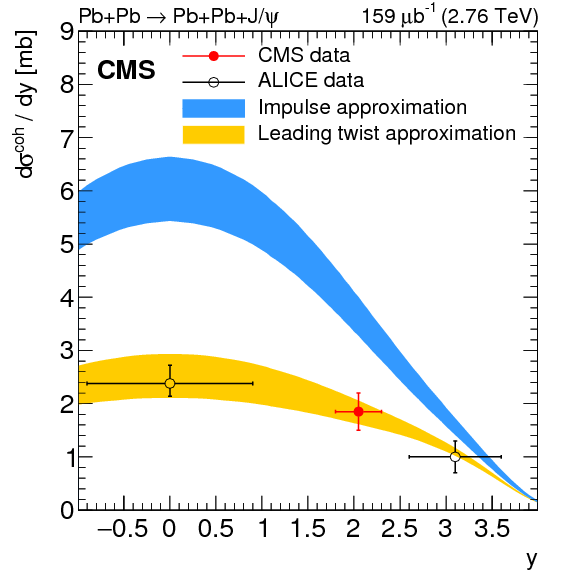
\includegraphics[width=4in]{Chapter2/importfigs/patkenny_Figure_002.png}
\par\end{centering}
\caption{Differential cross section versus rapidity for coherent $J/\Psi$ production in ultra-peripheral PbPb collisions at $\sqrt{s_{NN}}=2.76 TeV$ \cite{Khachatryan:2016qhq} \label{fig:pk3}}
\end{figure}
 
Studies of UPC $J/\Psi$ at CMS show that the measured cross section is consistent with models of the nucleus that include moderately strong gluon shadowing, in particular EPSO9 \cite{lta2013.05}\cite{Eskola:2009uj}. Fig \ref{fig:pk3} compares the cross section measured by CMS and ALICE against theoretical models. In the data there is a clear difference from the Glauber model prediction. The cross sections indicate that, at the energy scale of the $J/\Psi$ mass, the nuclear gluon density is suppressed with respect to that of the proton \cite{Frankfurt:2011cs}. Further studies can be done using UPC $\upsilon$ \cite{pQCD2013.02}. 

\section{Photon-photon interactions}

Classical electrodynamics forbids the scattering of a photon off another photon. According to Maxwell's equations, charge and current distributions make linear contributions to the electric and magnetic fields. For example, the electric field generated by a grid of static charges is the sum of the electric fields of the each charge considered by itself. This properpty, called "the principle of superposition", allows Maxwell's equations to be solved as boundary values problems via the separation of variables.

The cross section of a final state from the photon-photon interaction is given by
\begin{equation}
\sigma_X = \int d \omega_1 d \omega_2 \frac{n(\omega_1)}{\omega_2} \sigma_X^{\gamma\gamma}(\omega_1, \omega_2),
\end{equation}
where the subscripts $1$ and $2$ designate the quasi-real photons that are colliding and 
$\sigma_X^{\gamma\gamma}(\omega_1, \omega_2)$ is the cross-section of the final state from a collision of photons with energies $\omega_1$ and $\omega_2$. Once more, notice that the total final state cross-section is an integral of the all the photon energies in the photon flux. 

Maxwell's equations, being a classical theory, do not take into account the quantum mechanical effects that manifest at the distance scales of sub-atomic particles. The polarization of the vacuum is one such consequence of quantum mechanics. Around a photon there is a cloud of particle-antiparticle pairs, appearing together and then annihilating each other after a time proportional to their energy. In so far as these particles have an electric charge, portions of the local area may carry a non-zero electric charge. Thus, two photons may scatter off each other in three possible exchanges: Diagrams for Delbrück scattering, photon splitting, and elastic light-by-light scattering. 
\begin{figure}[h!]
\begin{centering}
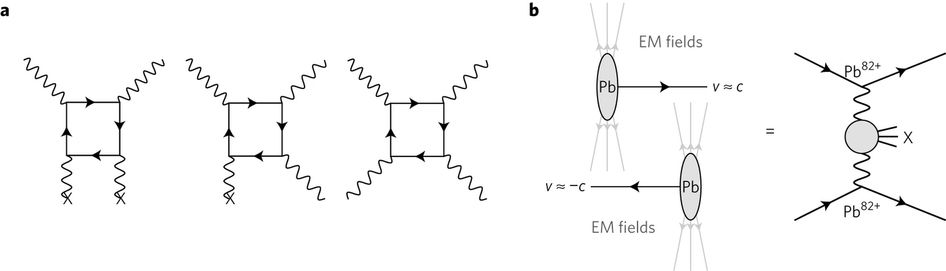
\includegraphics[width=7in]{Chapter2/importfigs/nphys4208-f1.jpg}
\par\end{centering}
\caption{$\gamma \gamma$ Diagrams of light-by-light scattering, (a.) channels, (b.) analagous \cite{Aaboud:2017bwk} \label{fig:ggDiag}}
\end{figure}

Figure \ref{fig:ggDiag} illustrates the process of light-by-light scattering. The plots in figure \ref{fig:ggDiag} (a.) are the Feynman diagrams of the three light-by-light channels: Delbruck scattering, photon splitting, and elastic scattering, respectively. Notice that all three channels are variations on a closed electron-loop. Figure \ref{fig:ggDiag} (b.) shows how these processes arise in heavy-ion collisions. The photon flux from a relativistic heavy-ion is calculated from the Fourier transform of its electric field. The final state $X$ is empty except for two photons \cite{Aaboud:2017bwk}. 
\begin{figure}[h!]
\begin{centering}
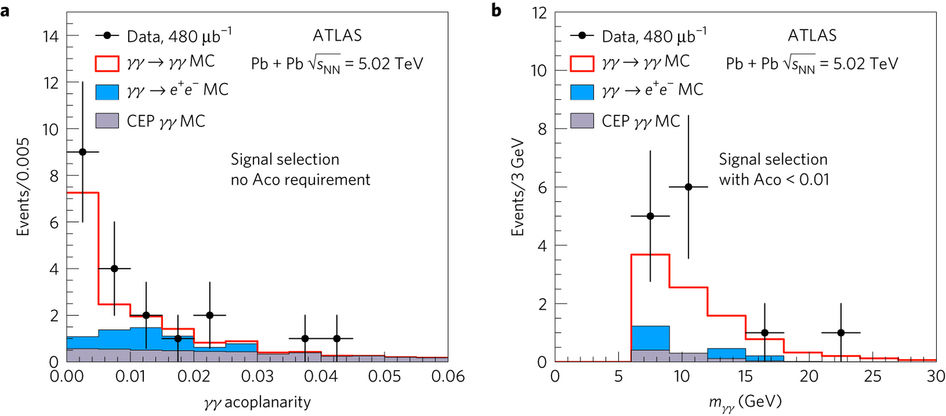
\includegraphics[width=7in]{Chapter2/importfigs/nphys4208-f3.jpg}
\par\end{centering}
\caption{$\gamma \gamma$ kinematics, (a.) acoplanarity, (b.) invariant mass \cite{Aaboud:2017bwk} \label{fig:ggKin}}
\end{figure}

Light-by-light scattering has been observed at ATLAS. The relevant data sample contains 480 $\mu b^-1$ of Pb+Pb data taken at $\sqrt{s_{NN}}=5.02$ TeV. Light-by-light MC was generated using STARLIGHT and processed through a GEANT4 simulation of ATLAS. The reconstructed MC was used to create kinematic templates for comparison against the data. These templates can be seen in figure \ref{fig:ggKin}. The most important part of the event selection is the cut on diphoton acoplanarity. 

\begin{figure}[h!]
\begin{centering}
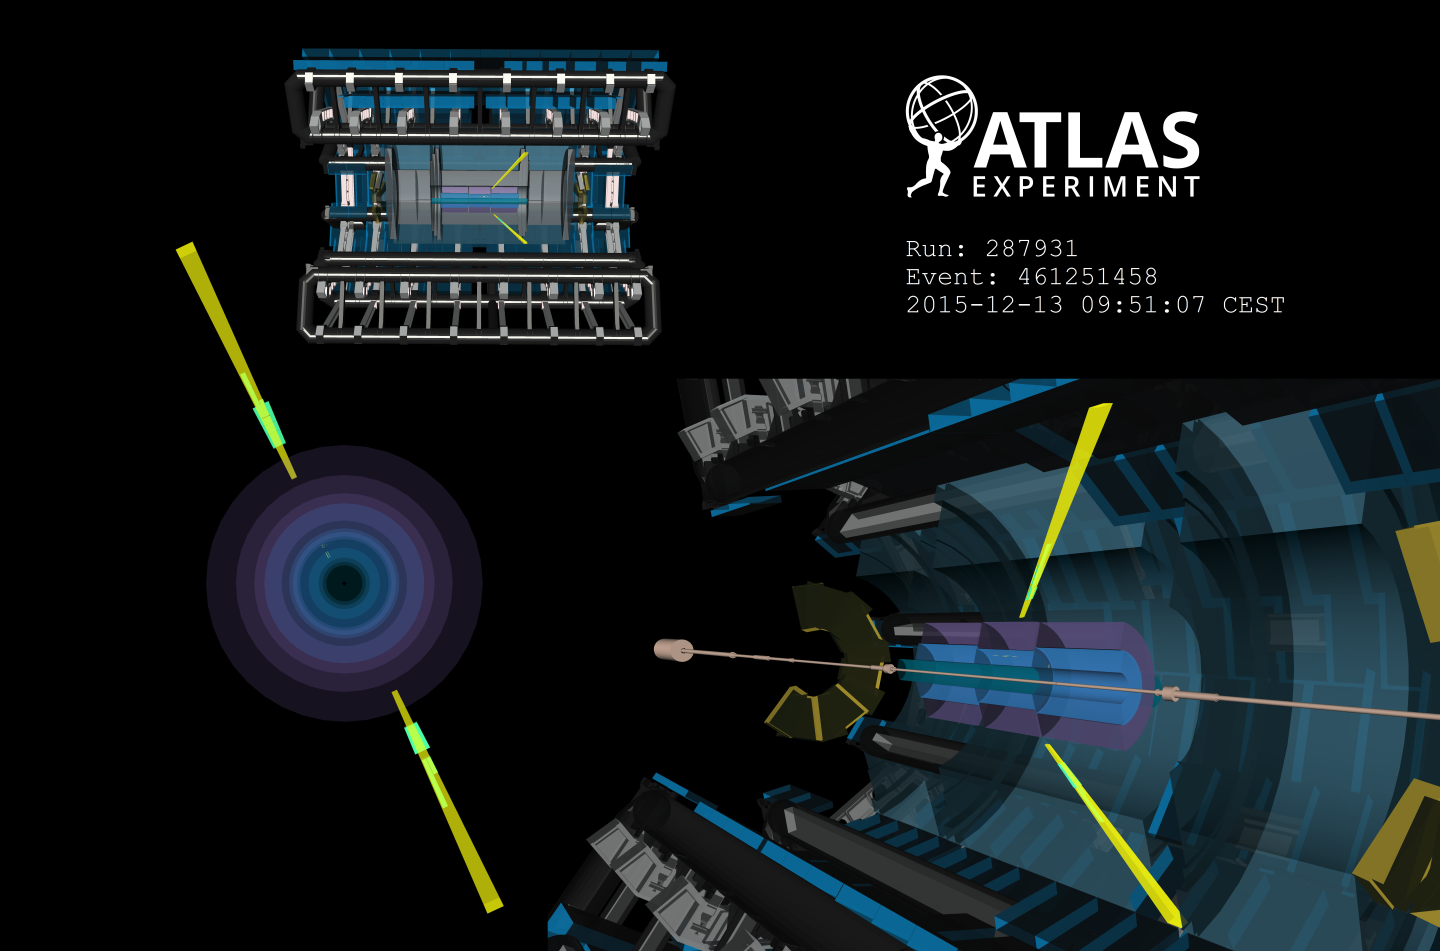
\includegraphics[width=5in]{Chapter2/importfigs/light-by-light-figure_2.png}
\par\end{centering}
\caption{Event Display of ATLAS photon-photon scattering \cite{Collaboration:2278547} \label{fig:atlasEvent}}
\end{figure}

Figure \ref{fig:atlasEvent} is an event display for an ATLAS light-by-light candidate \cite{Collaboration:2278547}. Notice that the two photons are back-to-back in the plane perpendicular to the beam.

\section{Dijet photoproduction}

Jets are one of the most interesting nuclear phenomena discovered in the modern era of particle acclerators. The existence of jets is a direct result of QCD confinement. In hadron collisions, it is possible for the hadron's constituent partons to fragment away. These partons, of themselves, would not be colorless. However, QCD confinement -- caused by the running QCD coupling -- demands that only colorless objects can independently exist. Therefore, as the fragment partons separate, they manifest new partons around themselves and screen the color charge. The formation of colorless composites, out of colored partons, is called "hadronization". The process of hadronization continues until the kinetic energy of all the fragmented partons drops below the potential energy the binding strong force. The result is a narrow cone of hadrons fanning out from a common source: a "jet". Analyzing a jet can elucidate the properties of its mother parton.  

An important experimental signature of deconfinement is how it affects hard-scattering processes. In a hard scattering process, partons are fragmented off from the nucleus and, due to confinement, hadronize into a cone of correlated final state particles, known as a jet. In theory, a jet should be sensitive to the medium that the mothering parton passes through. However, in order to detect the modification of a jet due to its mother parton passing through QGP, one needs a precise measurement of the jet production in of nuclear PDFs but not QGP. One can then determine QGP effects by comparison to the nuclear PDF baseline. However, there is a significant lack of data for low-x nuclear PDF. As Bjorken-x decreases, the nuclear PDF passes through stages three stages: EMC effects, anti-shadowing, and shadowing. EMC effects and shadowing are suppressions of the nuclear PDF in comparison to the proton PDF; anti-shadowing, by contrast, is the enhancment of the nuclear PDF in comparison to the proton PDF. 

The dijet photoproduction cross-section, like that of vector meson photoproduction, displays diffractive dips in its $|t|$ dependence. Furthermore, according to the color glass condensate formalism, coherent dijet production is sensitive to gluon saturation effects at small Bjorken-x values \cite{Guzey:2016awf}\cite{Guzey:2016tek}. Gluon saturation would affect the color-dipole orientation of nucleons in the transverse plane. This effect should be reflected in an enhanced azimuthal angle correlation of the jets. 

ATLAS has published preliminary results on UPC dijet production. It has been shown that these photonuclear dijets manifest distinct differences from dijets produced in more "hadronic" collisions. There are rapidity gaps that are similar to those seen in the diffractive productions of electron-proton collisions at HERA. The forward neutron emission spectrum also matches that expected for UPC data set. The ATLAS results are particularly interesting because Strikman, Vogt, and White have shown that UPC dijet photoproduction is sensitive to the low Bjorken-x nuclear PDFs.

ATLAS used a combination of triggering, forward calorimetry, and rapidity gap requirements to select events of photo-nuclear dijet production in ultra-peripheral heavy-ion collisions. Figure \ref{fig:exampleDijetAtlas} shows the two variations of the leading order diagram for UPC dijet production. On the left is direct photo-production, in which the mediating virtual photon has low enough virtuality to interact with the nucleus as a photon. On the right is resolved photo-production, in which the virtual photon has a high enough virtuality to manifest a hadronic structure, the interaction with the nucleus is mediated by a pomeron. Directly photo-produced final state particles will have a characteristic rapidity gap in the final state because the target nucleus does not dissociate. Resolved photoproduction, however, excites the nucleus such that the rapidity gap is partially filled. 
\begin{figure}%
    \centering
    \subfloat[label 1]{{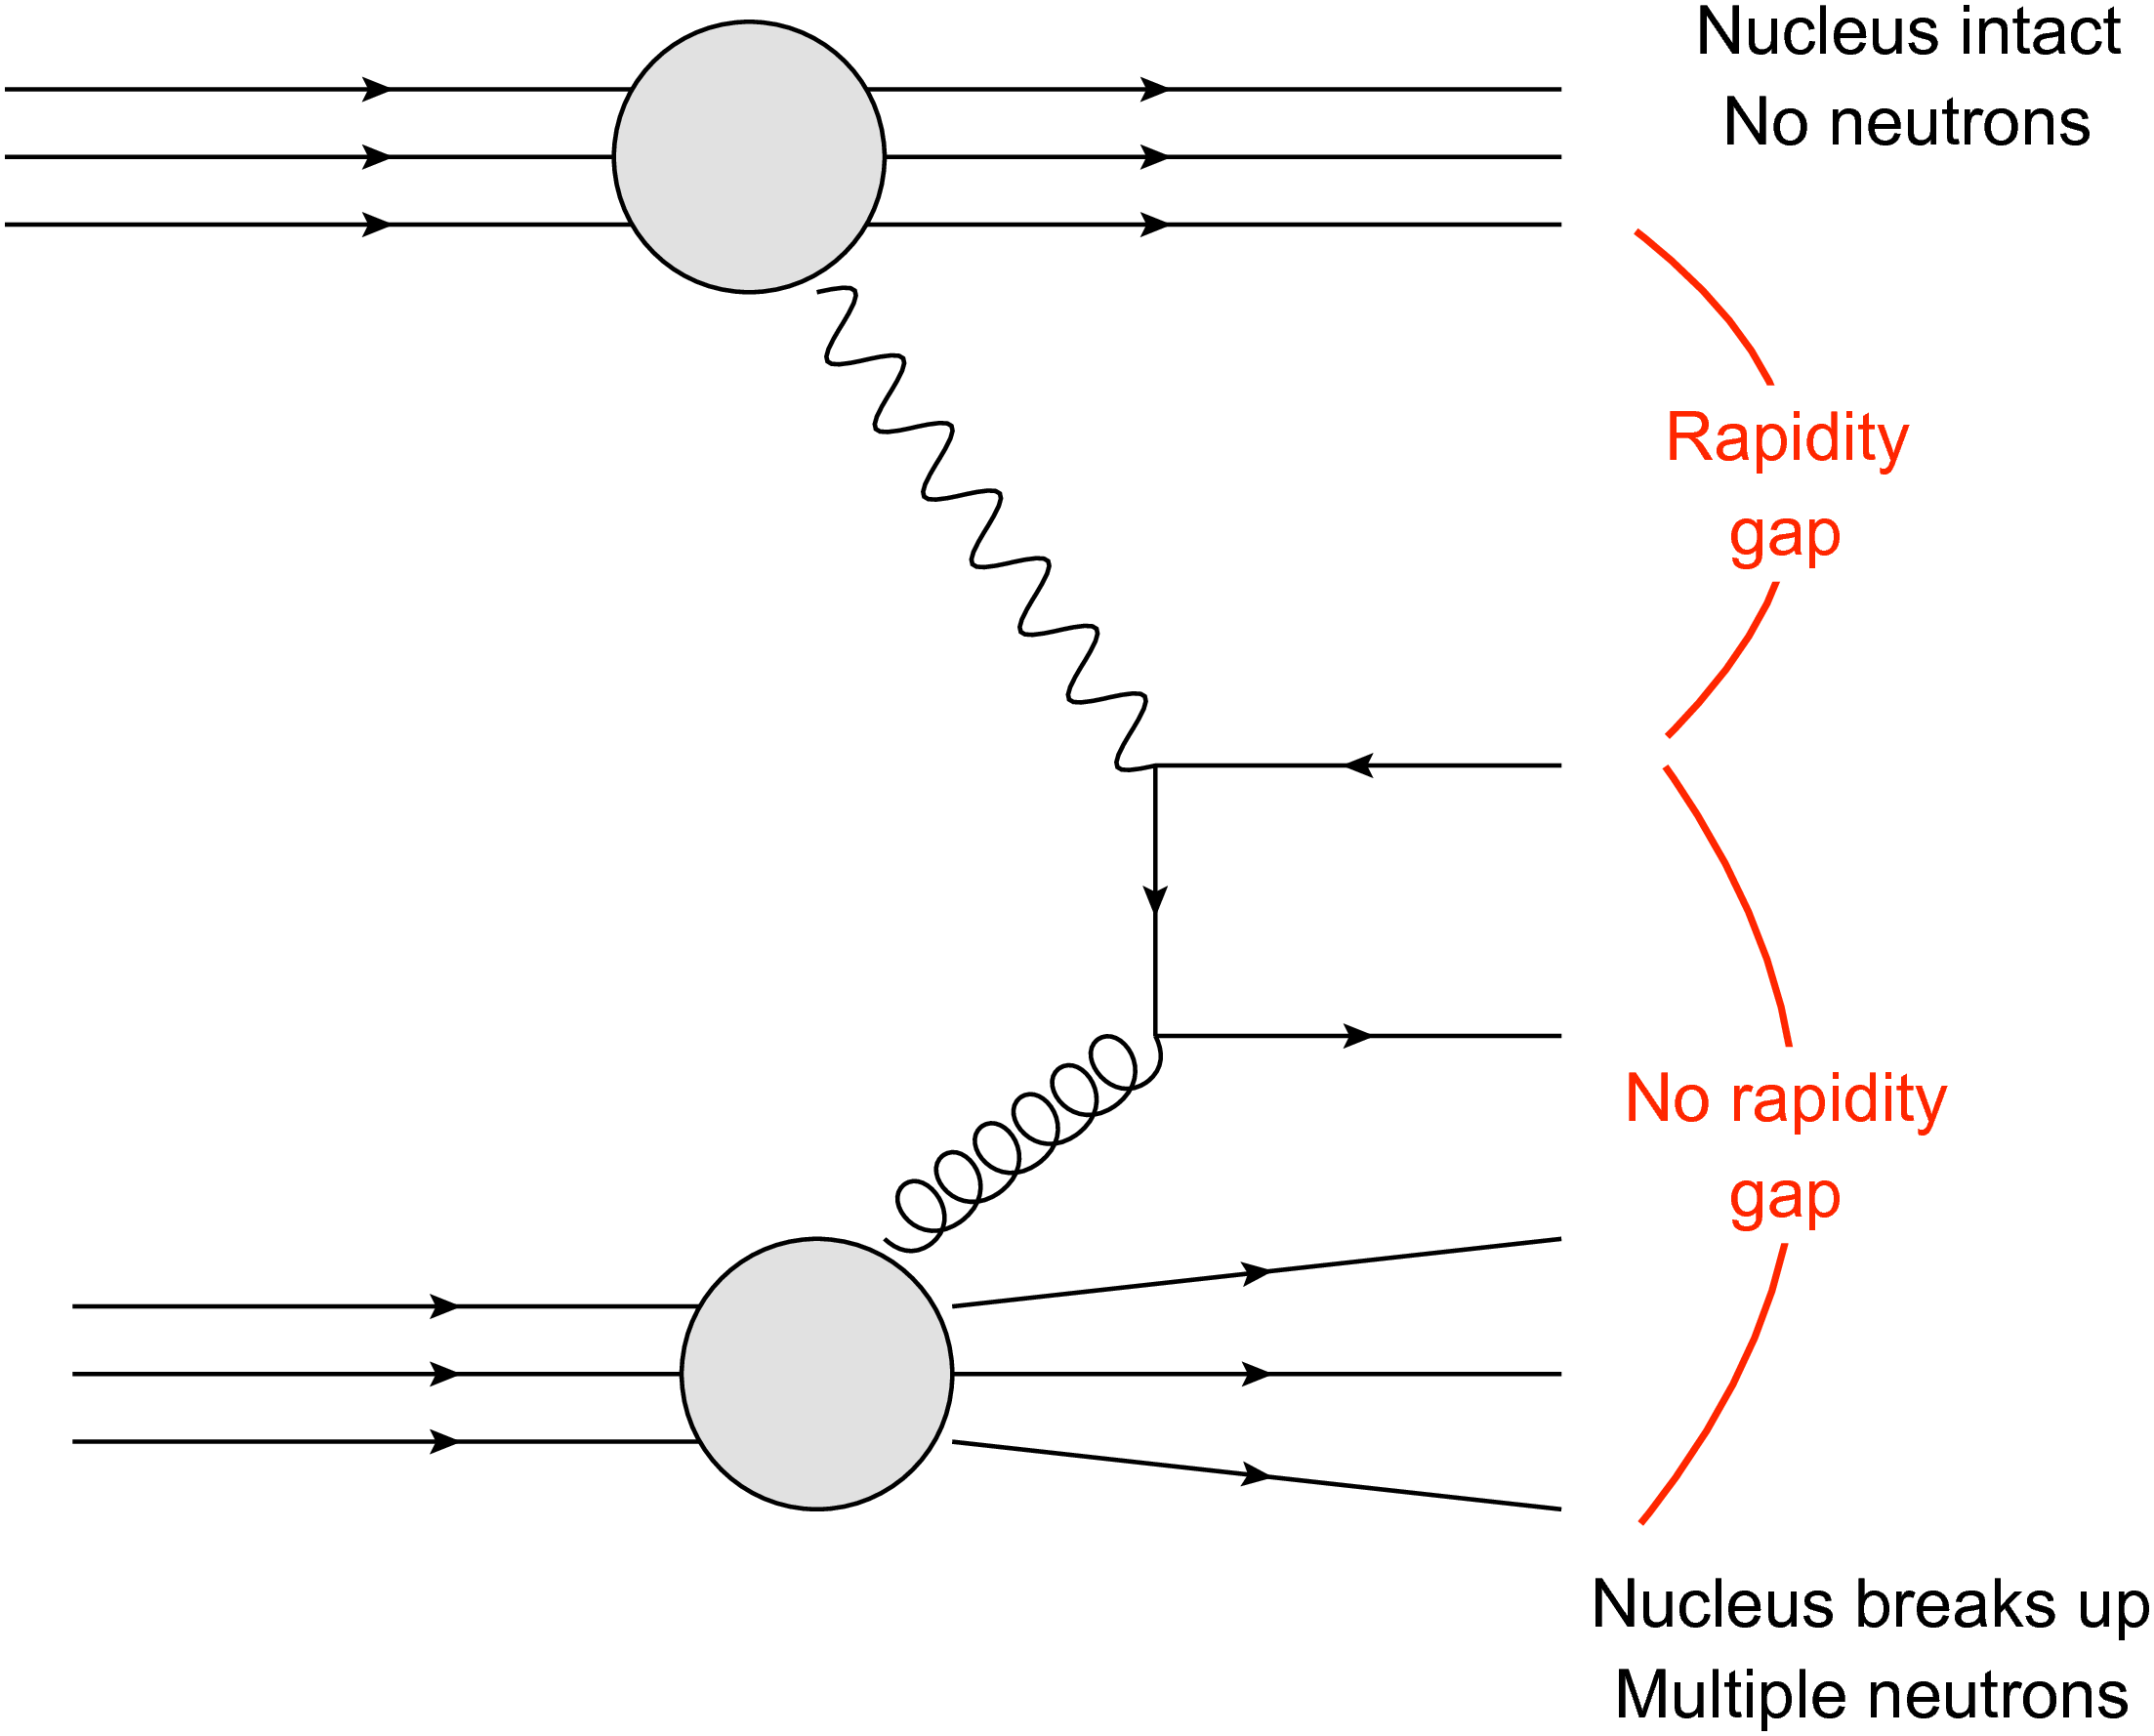
\includegraphics[width=6cm]{Chapter2/importfigs/fig_01a.png} }}%
    \qquad
    \subfloat[label 2]{{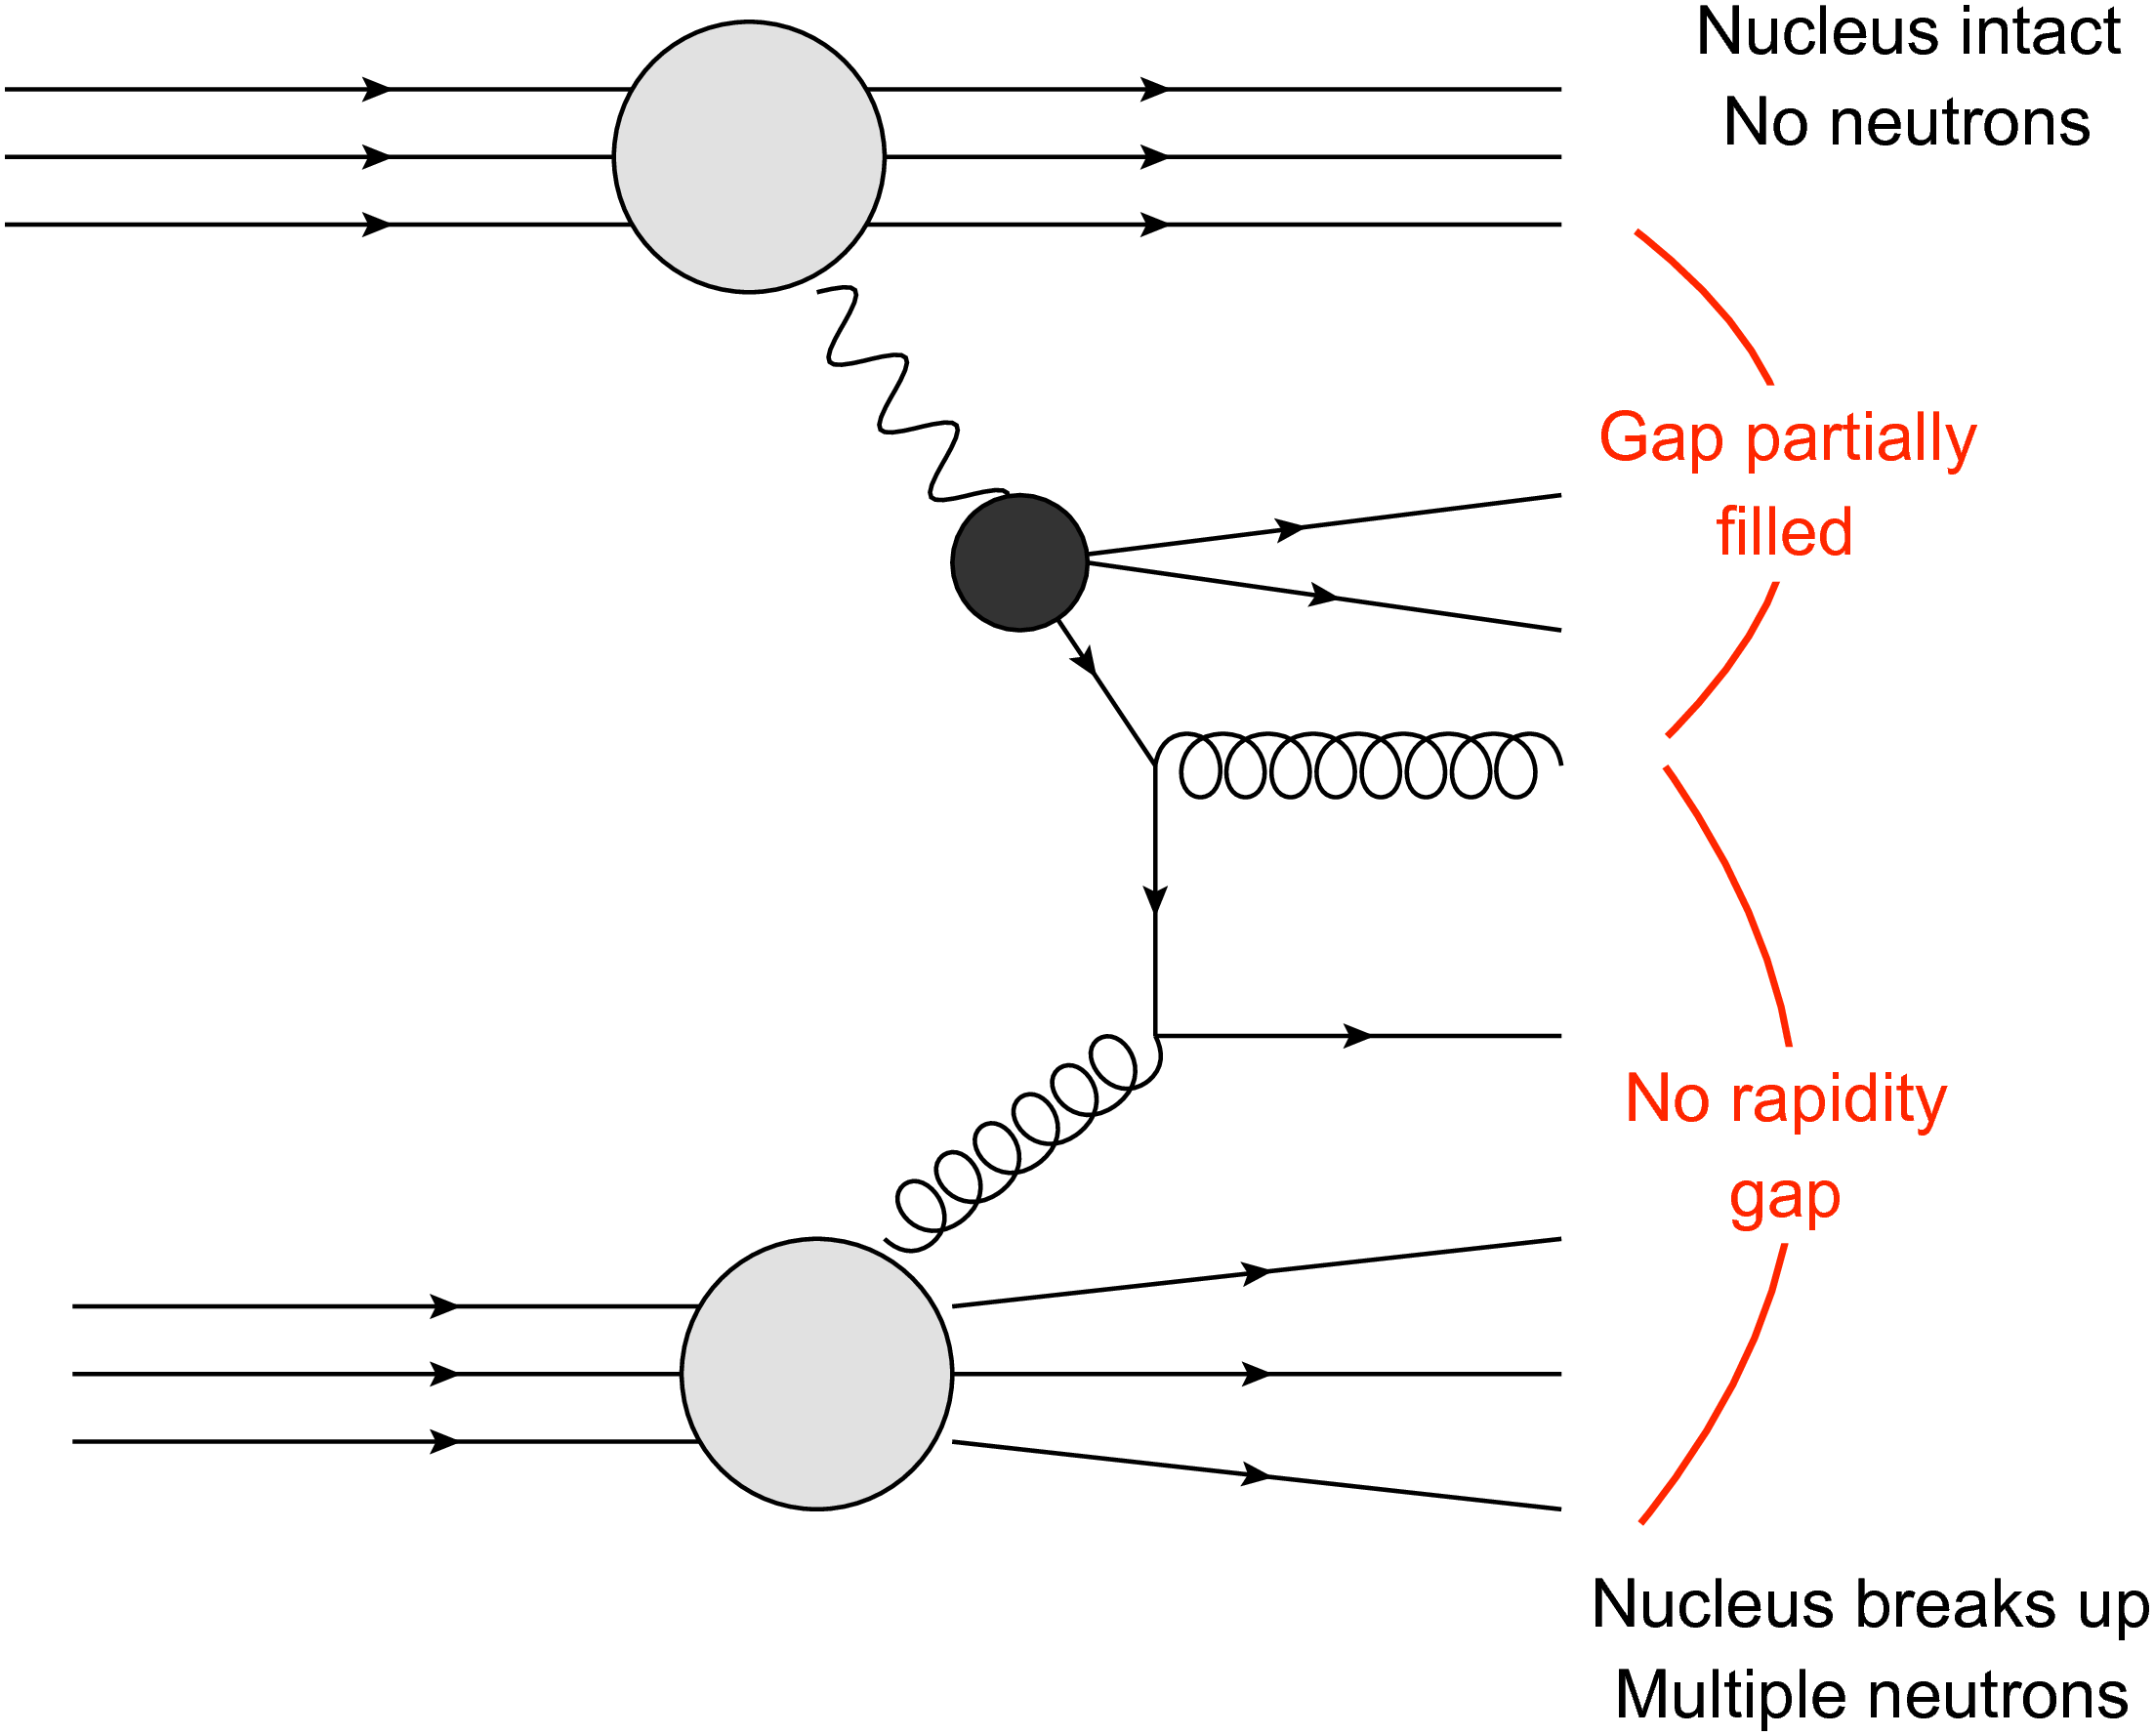
\includegraphics[width=6cm]{Chapter2/importfigs/fig_01b.png} }}%
    \caption{2 Figures side by side}%
    \label{fig:exampleDijetAtlas}%
\end{figure}

ATLAS reported the cross-section of photo-nuclear dijet production versus various dijet kinematic variables, and compared these cross-sections to those derived from MC. The MC sample was generated by Pythia and re-weighed to fit the quasi-real photon spectrum of a relativistic Pb ion. The photon spectrum itself is taken from the STARLight MC generator.

\subsection{Factorization}

Diffractive dijet photoproduction is not describable in perturbative QCD. For coherent processes the photon energy is small, and therefore the wavelength is large compared to the size of the nucleus. At these large distances, there isn't a hard scale, and so perturbation calculations cannot be done. Gluon splitting interactions dominate the low Bjorken-x partons. QCD collinear factorization describes these soft interactions via the convolution of parton cross sections, taken from perturbative QCD, and diffractive parton distribution functions, taken from experiment \cite{Andreev:2015cwa} \cite{Chekanov:2008fh}. The photon can interact directly with the nucleon, or the photon can fluctuate into a quark-antiquark pair which interacts with the nucleon. The resolved-photon has a hadronic structure and its own corresponding PDF \cite{Bauer:1977iq}.
\begin{figure}[h!]
\begin{centering}
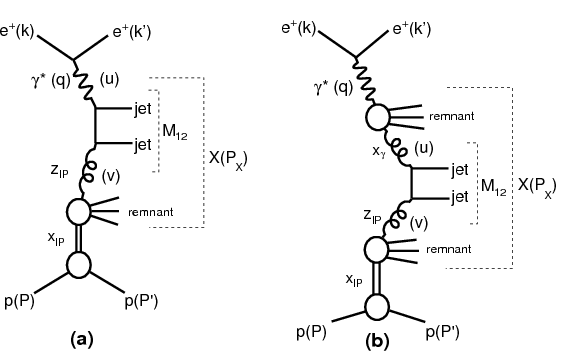
\includegraphics[width=6in]{Chapter1/importfigs/h1_2015_feyn.png}
\par\end{centering}
\caption{Feynman diagrams for coherent jet photoproduction in (a) direct-photon in ep, (b) resolved-photon in ep \cite{Andreev:2015cwa} \label{fig:feynmanUPC1}}
\end{figure}

In electron-hadron collisions, diffractive photoproduction is characterized by the presence of a large rapidity gap in the final state and an intact nucleus \cite{Frankfurt:2006tp}. The Feynman diagram of electroproduction in lepton-hadron collisions is similar to that of photoproduction in ultraperipheral collisions, as seen in figure \ref{fig:feynmanUPC1} \cite{Andreev:2015cwa}. The large rapidity gap here is due to the leading proton \cite{Aaron:2010aa}. The diffractive dijet cross section is expressed by the convolution of partonic cross sections $d\hat{\sigma}$ and diffractive PDFs $f^D_{i/p}$.
\begin{equation}
d\sigma (ep \rightarrow e + 2 jets + X^{'} + p) = \sum_{i} \int dt \int dx_\mathbb{P} \int dz_\mathbb{P}d\hat{\sigma}_{ei\rightarrow 2jets}(\hat{s},\mu^2_R,\mu^2_F)\times f^D_{i/p}(z_\mathbb{P},\mu^2_F,x_\mathbb{P},t) ,
\end{equation}
where $x_\mathbb{P}$ is longitudinal momenetum fraction lost by the incoming proton, $d\hat{\sigma}_{ei\rightarrow 2jets}$ is the partonic cross-section for the process, $z_\mathbb{P}$ is the longitudinal momentum fraction of the pomeron entering the hard process, $\hat{s}$ is the squared invariant energy of the subprocess, $\mu^2_R$ is the squared renormanlization scale, $\mu^2_F$ is the squared factorisation scale, $f^D_{i/p}$ is the diffractive parton distribution,and $t$ is the four-momentum transfer squared at the vertex. 

In the proton-vertex factorisation hypothesis, the dependence on $x_{\mathbb{P}}$ and $|t|$ is factored out of the dependence on $\mu^2_F$ and $z_{\mathbb{P}}$. Furthermore, $f^D_{i/p}$ is sum of contributions from the pomeron and Reggeon:
\begin{equation}
f^D_{i/p}(z_{\mathbb{P}},\mu^2_F,x_{\mathbb{P}},t) = f_{\mathbb{P}/p}(x_{\mathbb{P}},t)f_{i/\mathbb{P}}(z_{\mathbb{P}},\mu^2_F) + n_\mathbb{R}f_{\mathbb{R}/p}(x_{\mathbb{P}},t)f_{i/\mathbb{R}}(z_{\mathbb{P}},
\mu^2_F) ,
\end{equation}
where $_{\mathbb{P}/p}$ is the pomeron flux factor, $f_{\mathbb{R}/p}$ is the Reggeon flux factor, $n_\mathbb{R}$ is the normalization factor of the Reggeon, $f_{i/\mathbb{P}}$ is the pomeron parton distribution, and $f_{i/\mathbb{R}}$ is the Reggeon parton distribution.

Lepton-hadron collisions were performed at HERA and measured by the H1 experiment. These experiments reported a value for the total diffractive photoproduction cross section that is double that predicted by QCD collinear factorization; figure \ref{fig:h1Ratio} compares the cross-section of H1 data to that predicted by NLO-QCD \cite{Andreev:2015cwa}. Diffractive events were selected for using rapidity gaps or the presence of leading protons in the very forward proton spectrometer (VFPS). 

\begin{figure}[h!]
\begin{centering}
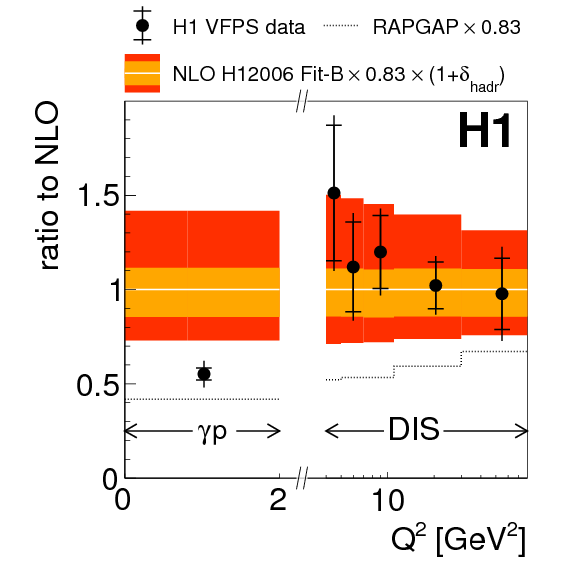
\includegraphics[width=3in]{Chapter1/importfigs/fig8_h1_2015.png}
\par\end{centering}
\caption{Ratio of H1 data cross-section to NLO-QCD cross-section \cite{Andreev:2015cwa} \label{fig:h1Ratio}}
\end{figure}

H1 used the Very Forward Proton Spectrometer (VFPS) to trigger on low $Q^2$ protons. The VFPS consists of two Roman Pots located 218 m and 222 m from the H1 interaction-point in the forward direction. The VFPS can detect protons scattered at very low transverse momentum, corresponding to $0.008 < x_{P} < 0.028$ and $|t|<0.6$. Each of the Roman Pots contains layers of scintillating fibers, which are covered by a layer of scintillator tiles. The fibers readout to photomultipliers, and the tiles both shield from radiation and trigger on protons. The track effiency of VFPS is a remarkable $96 \%$, and the background contamination is kept at $1 \%$ , making the detector excellent for studying diffractive events. Figure \ref{fig:h1BeamEnv} shows the $|t|$ coverage of the Forward Proton Spectrometer (FPS) and VFPS \cite{Andreev:2015cwa}.

\begin{figure}[h!]
\begin{centering}
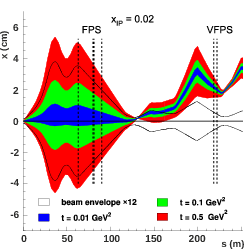
\includegraphics[width=3in]{Chapter1/importfigs/fig7_h1_2015.png}
\par\end{centering}
\caption{Beam envelope vs. distance to vertex in H1 \cite{Andreev:2015cwa} \label{fig:h1BeamEnv}}
\end{figure}

The H1 data was compared to predictions based on NLO-QCD convoluted with diffractive parton distribution functions (DPDFs) from HERA inclusive diffractive deep-inelastic scattering (DDIS) data. For diffractive pp collisions the high transverse momentum jets yield a hard scale for perturbative QCD \cite{Aaron:2010su}. 

